\documentclass[12pt,fleqn]{article}\usepackage{../common}
\begin{document}
Ders 10

Bu dersin konusu sal�n�mlar (oscillations), ki bu kavram gunluk hayatta
surekli kar��la��lan ve onemli bir kavramdir. Bizim onceden gordugumuz
sal�n�mlar karakteristik denklem $r^2 + br + k = 0$'in kompleks kokleri ile
alakaliydi. Kompleks kokler 

\[ r = a \pm bi \]

formundadirlar. 

[onceki derste $a$ ve $b$ reel kisimlari kullanmak yerine niye $a$ ve $-b$
kullanmanin gereksiz oldugu hakkindaki bolum atlandi].

Su resme donelim. 

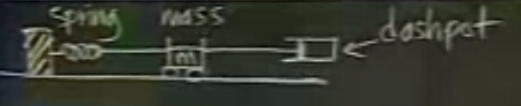
\includegraphics[height=2cm]{10_1.png}

Formuller

\[ mx'' + cx' + kx = 0 \]

\[ x'' + \frac{c}{m}x' + \frac{k}{m}x = 0 \]

En alttaki standart form. Bu formulu degisik bir sekilde yazalim - hem
eklektik [farkli seylerin birlesimi], hem degisiklik olsun diye, boylece
$x$ bazli kullanima fazla bagli olmayiz, her turlu kullanimla is
yapabiliriz. Soyle bir form kullanalim:

\[ y'' + 2p y' + \omega_0^2y = 0 \]

Niye 2 ve niye $\omega_0$'in karesini kullandigimizi ileride anlayacagiz
(bu sekilde kullanim bazi ilgili formullerin daha temiz olmasini sagliyor).

Biz bu derste salinimlarla ilgilendigimiz icin ustteki formulun kompleks
kokleri oldugu kosullarla ilgileniyoruz, eger kokler reel olsaydi o zaman
sistem fazla amortisorlu (overdamped) olurdu, bu durumla
ilgilenmiyoruz. Genel olarak ta amortisorsuz durum daha cok ilgi ceken bir
durumdur.

Karakteristik denklem nedir?

\[ r^2 + 2pr + \omega_0^2 \]

$p$ bir sabit, cogunlukla denklemde o pozisyondaki bir $p$ degiskenini
$p(t)$ seklinde kullaniyordum, ama burada $p$ sabit. 

Denklemin kokleri nedir? Simdi $p$'nin onune bir 2 koymanin faydalarini
goruyoruz herhalde, karesel cozum denklemi:

\[ \frac{-b \pm \sqrt{b^2-4ac}}{2a} \]

Birinci kisim, $a=1$ olduguna gore $-b / 2$, o zaman $-2p / 2 = -p$. 2 
sayesinde temiz bir sonuc oldu. $\sqrt{b^2-4ac} / 2$ icin bolumun ustu 
$\sqrt{4p^2 - 4\omega_0^2}$, karekok icindeki 4'ler disari 2 olarak cikabilirler, 
cikinca da bolen 2 ile iptal olabilirler. Geriye $\sqrt{p^2 -
  \omega_0^2}$ kalir. Sonucun 
tamami

\[ -p \pm \sqrt{p^2 - \omega_0^2} \]

Yani bir karesel denklemde matematikciler ikinci terime ne zaman bir 2
yerlestirirlerse, bunu yapmalarinin sebebi karesel cozum formulunu
kullanmak istemeleri ve ekstra 2 sayilarinin formulu karistirmasini
engellemek istemeleridir.  

Eger $p=0$, yani $c/m = 0$, yani ortada engelleyici yok. Bu amortisorsuz
(undamped) durum. O zaman o terim yokolunca geri kalan denklem

\[ y'' + \omega_0^2y = 0 \]

Bu basit harmonik hareket (simple harmonic motion) denklemidir, ki
ogrenciler bu denklemi zaten ustteki gibi gormeye alisiktir. Niye? Cunku o
zaman $\omega_0$ terimi salinimin dairesel frekansini temsil eden
terimdir. O formdaki bir denkleme bakarak aninda frekansin ne oldugunu
cikartabilmis oluruz. 

Genel cozumler o zaman $r=\pm i \omega_0$ seklinde olurlar, kompleks
acilimi kullanirsak 

\[ y = c_1 \cos(\omega_0 t) + c_2 i\sin (\omega_0 t) \]

ya da

\[ y = A \cos(\omega_0 t - \phi) \]

Tum bunlar $k/n$ yerine niye $\omega_0$'in karesini kullandigimizi
ispatlamistir herhalde. Simdi sorumuz amortisorlu kosulun neye
benzeyecegi. Bu durum probleme biraz daha yakindan bakmayi ve daha fazla
dusunmeyi gerektiriyor. 

Amortisorlu kosulu dusunelim. Bu sistemde ne zaman salinim elde ederim?
$\sqrt{p^2 - \omega_0^2}$'in ici negatif oldugu zaman, yani $p^2 -
\omega_0^2 < 0$. Ayrica $p$ ve $\omega_0$'in 
pozitif olmasi mecbur olduguna gore (cunku oyle tanimladik) gore o zaman 
$p
< \omega_0$ olmalidir. 

Bu kosulu konusma ile belirtmek gerekirse, ``amortisor terimi dairesel
frekanstan kucuk oldugu zaman''. Tabii amortisorun yarisi demek istiyoruz
aslinda cunku $p$'yi 2 ile carptik, bir de orijinal formulde $m$ ile bolum
var, bunu da hesaba katmali. Yani, belki amortisor yerine $p$ demek daha
dogru olur.

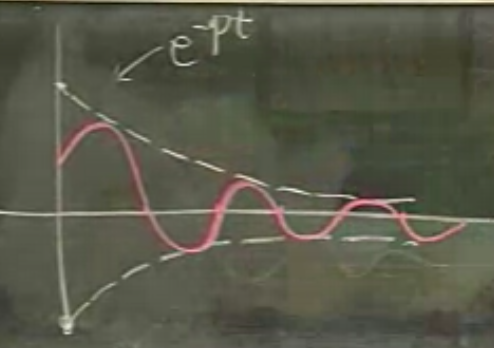
\includegraphics[height=4cm]{10_2.png}

Onceki dersten hatirlarsak, cozumun grafigi usttekine benzer. Ozel
(particular) cozum kirmizi cizgidir, y eksenini kestigi nokta baslangic
sarti tarafindan tanimlanir, altinda kaldigi $e^{-pt}$ egrisi onun bir nevi
yuksekligidir (amplitude). 

Bu noktada sorulabilecek ilk ilginc sorulardan biri, cozumun t eksenini
kestigi her noktanin arasindaki bosluk nedir? 

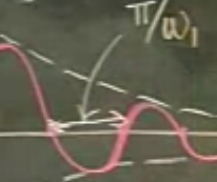
\includegraphics[height=2cm]{10_3.png}


Bu mesafe, yani periyotun buyuklugunu $\pi / \omega_1$ olarak belirtelim,
$\pi$ cunku hemen yanindaki parcayi da dahil etseydik o nokta bir salinimin
tamamlandigi noktadir, orada $2\pi$ kullanilacakti. Genel baglamda bu
fonksiyon aslinda yari-periyodik diye nitelenen fonksiyonlardan, tam
periyodik degil cunku fonksiyonun yuksekligi surekli azaliyor ama periyodik
``olmaya ugrasiyor'', en azindan bir seyi periyodik olarak yapiyor, t
eksenini periyodik olarak kesiyor. $\omega_1$ frekans, ama ona aslinda
``yari (pseudo) frekans'' demek lazim, aynen fonksiyonun ``yari-periyodik''
olmasi gibi.

Sezgisel olarak dusunelim: Eger amortisor $c$ artarsa, yari-frekans
$\omega_1$'e ne olur? Duser. Simdi formulsel olarak dusunelim. $\omega_1$
nedir? Ana denklemin cozumune bakalim

\[ r = -p \pm \sqrt{-(\omega_0^2 - p^2)} = -p \pm \sqrt{-\omega_1^2}\]

$(\omega_0^2-p^2)$ parentezi disina bir eksi isareti koydum, cunku o terimin
negatif bir sayi oldugunu vurgulamak istedim, $\omega_0^2-p^2$ ifadesinin
karesi elimizdeki yeni frekans olacak. 

Burada yeni frekans $\omega_1$ olacaktir, cozumu yazalim, ve $\omega_1$'in
karesinin karekoku yine kendisidir, ama onundeki eksinin karekok disina
cikarken bir $i$ ortaya cikartacagini hesaba alarak

\[ e^{-pt}(c_1 \cos \omega_1 t + c_2 \sin \omega_1 t) \]

ya da 

\begin{equation}\label{eq1}
 e^{-pt} A \cos (\omega_1 t - \phi) 
\end{equation}

ve boylece $\omega_1$'in yari-frekans oldugunu goruyoruz. Niye? Cozumun t
eksenini kestigi ilk yeri $t_1$ olarak dusunelim. O zaman $t_2$ nedir? 
$t_2
= t_1 + 2\pi / w_1$. Degil mi? t eksenini kesmek demek $cos (\omega_1 t -
\phi)$ 
ibaresinin sifir olmasi, bir cos teriminin sifir olmasi ise
$\pi/2$'nin katlarinda oldugumuzu gosterir.  

\[ \omega_1 t - \phi = \pi / 2 \]

Bir dahaki kesisme

\[ \omega_2 (t_1 + \frac{2\pi}{\omega_1}) - \phi = \pi / 2 + 2\pi\]

Simdi formul \ref{eq1}'de neyin neye bagli oldugunu gormek
istiyorum. Elimizdekiler sunlar: $p$, $\phi$, $A$, $\omega_1$.

$p$: sadece ODE'ye bagli ($c/2m$)

$\phi$: Baslangic kosullarina bagli

$A$: Baslangic kosullarina bagli

$\omega_1$: sadece ODE'ye bagli. $\omega_1$'i iceren formul neydi?
$\omega_0^2 - p^2  = \omega_1^2$. Bu Pitagor'un Teoremi ile alakali, sekil altta.
$\omega_1$ amortisor, o zaman yaya, yani yay sabitine bagli. 

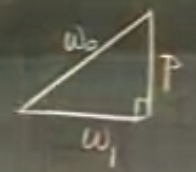
\includegraphics[height=2cm]{10_4.png}



\end{document}





